%% notes-tex/019-simb-multimodal-expression/019-simb-multimodal-expression.tex
%% [[experiments.019-simb-multimodal.expression-strand-retrospective]]
%% https://github.com/Mjvolk3/torchcell/tree/main/notes-tex/019-simb-multimodal-expression/019-simb-multimodal-expression.tex
%%
%% Typeset counterpart of notes/experiments.019-simb-multimodal.expression-strand-retrospective.md,
%% the running record of the EXPRESSION strand after the SIMB sprint. The six-strand
%% retrospective (notes-tex/019-simb-multimodal/) stays as reviewed; everything that
%% happened to expression after its launch section lives here.
%%
%% Build:  make            -> 019-simb-multimodal-expression.pdf         (draft: status chips + provenance flags)
%%         make clean-view -> 019-simb-multimodal-expression-clean.pdf   (share view)
%%         make check      -> formatting / provenance gate
%%         make plots      -> refresh figures/ from the plot scripts' true-size SVGs
%%
%% EVERY number in this document comes from a committed script under experiments/ or
%% from a named W&B run id or slurm job id, and is marked with a `%% SOURCE:` comment.

\documentclass[10pt,a4paper]{article}
\usepackage[draft]{tcdoc}

\title{\vspace{-1.5em}Expression After SIMB\\
  {\large The Knockout-Expression Strand: What the Campaign Established,\\
   Read Round by Round}}
\author{Michael Volk}
\date{\today}

\begin{document}
\maketitle
\thispagestyle{empty}

\begin{abstract}
\noindent
One strand of the SIMB retrospective, knockout expression on Kemmeren and Sameith, became
the campaign that followed it: four rounds on IGB and Delta between 2026-08-31 and
2026-09-08, all under the masked-label objective of project \file{torchcell_019_expr_v9}.
Every score is one statistic, the maximum of a centered 5-epoch rolling mean of the
per-gene validation Pearson, read from the full history of every run and placed against
eight identical-config replicates of the incumbent, whose spread at the full budget is
$0.0222$ around a mean of $0.1965$.

What is established. The distributional head is not load-bearing: a point head collapses,
the CRPS head collapses two times in three, and the Laplace-CRPS head ties the quantile
head to $0.0005$. The validation loss bottoms out at a few hundred epochs in every run
while the metric keeps rising to beyond 19,000, so the long budget buys Pearson on a rising
objective. Training on the metric itself does not escape that: pure Pearson at batch 32
collapses to constant outputs at every seed, and the batch-64 variant that survives sits on
the incumbent band rather than above it. The one factor that moves the score by more than
the replicate spread is the content of the gene embedding, ProtT5 over random by $0.07$ at
1,000 epochs; trunk depth, readout width and weight decay do not. The per-gene readout is
$+0.03$ over its in-round reference at two seeds, under the resolution of that round, and
the pair term alone is a null. Four of four packed five-day tasks died of host memory.

What is not. Nothing measured beats the incumbent's replicate mean at any budget; the
incumbent's own embedding, \file{calm}, has not been placed against ProtT5; and no design
run so far resolves a gap under about $0.04$ at the full budget.
\end{abstract}

\vspace{0.5em}
{\small\color{tcgray}
\textbf{How to read this.} \cref{sec:findings} is the state of the strand: every claim with
its script, its statistic and its sample size, in the order the evidence arrived.
\cref{sec:readouts} is the readout of the three rounds that returned on 2026-09-08.
\cref{sec:next} is what the evidence leaves open. The design and launch of the rounds,
and the retrospective they grew out of, are in \file{notes-tex/019-simb-multimodal/}
(sections 9 and 10 there), which is not repeated here.\par\smallskip

Working note: \file{notes/experiments.019-simb-multimodal.expression-strand-retrospective.md}\par
Generating scripts: \file{experiments/019-simb-multimodal/scripts/}\par
Leaderboard: \file{experiments/019-simb-multimodal/results/round_leaderboards.csv}\par}

\vspace{1em}
\tccontents

\clearpage
%% notes-tex/019-simb-multimodal-expression/sections/1-findings.tex
%% SOURCE: experiments/019-simb-multimodal/results/round_leaderboards.csv and
%% round_leaderboards_summary.json (pull_round_leaderboards.py); short_budget_spread.json
%% (short_budget_spread.py); budget_rank_preservation.json (budget_rank_preservation.py);
%% loss_min_vs_pearson_peak.json (loss_min_vs_pearson_peak.py); expression_baselines
%% (expression_baselines.py); the objective-round table as read on 2026-09-06 and recorded
%% in notes/experiments.019-simb-multimodal.expression-strand-retrospective.md. The ceiling
%% is the replicate-based figure of the SIMB retrospective (section 2 there).

\section{The state of the strand, claim by claim\secstatus{todo}}
\label{sec:findings}

The task is the one of \cref{sec:strand-task}, scored by the per-gene Pearson across
held-out strains and averaged over genes against a replicate ceiling of $0.775$.
Everything below is read from the leaderboard puller (\file{pull_round_leaderboards.py}) over project
\file{torchcell_019_expr_v9}, which is the masked-label objective, or from a script named
in the paragraph. The statistic throughout is \file{roll_max}: the maximum of a centered
5-epoch rolling mean of \file{val/expression/pearson_per_feature}, an upward-biased order
statistic whose bias grows with the epochs run, and which cancels in a contrast between
runs scored the same way.

\subsection{The incumbent and its spread\secstatus{todo}}
\label{sec:findings-state}

The incumbent is the quantile head under the pinball loss, learning rate $3 \times 10^{-4}$,
dropout $0.1$, six transformer layers at hidden width 90, the nine-graph attention mask,
\file{calm} gene embeddings, batch 32, 9{,}900 epochs, and the reveal schedule
$[0, 10, 100, 1000]$. Eight runs at that budget share every one of those settings the
leaderboard records and score $\mathbf{0.1965 \pm 0.0222}$; they were read as
identical-config replicates until 2026-09-08, when their W\&B configs showed them to be the
eight arms of the v9 mask-schedule round (\texttt{M\_sched}, the incumbent schedule;
\texttt{M\_lo}, \texttt{M\_hi}, \texttt{M\_fine}, \texttt{M\_coarse}, other schedules;
\texttt{M\_nomix}, mixing off; \texttt{M\_gate\_rezero}, gate closed; \texttt{M\_off}, no
schedule). So $0.1965 \pm 0.0222$ is a mean and spread across arms, the spread bounding
nondeterminism from above; the incumbent schedule itself is one draw at $0.1824$, and the
three highest leaderboard entries, $0.238$ to $0.243$, are the \texttt{M\_fine} arm and its
resumed lineage to 19{,}000 epochs, one draw of one schedule. Replicate spread measured on
runs that do share a configuration is $0.0246$ pooled within cell at epochs $\le 990$
(\cref{sec:readouts-factorial}) and $0.019$ between two seeds of the mechanism-round
reference at epochs $\le 4{,}079$ (\cref{sec:readouts-mech}). Baselines that need no GPU
(\file{expression_baselines.py}): per-gene mean $0.0000$, bilinear on ProtT5 $0.1040$,
embedding-neighbor $0.0908$. The incumbent clears the bilinear by $0.093$, about $4.2$
standard deviations. On squared error no live run beats the per-gene mean at its Pearson
peak: the best \file{nmse} at peak is $1.005$.

\subsection{The head is not load-bearing\secstatus{todo}}
\label{sec:findings-head}

The objective round (IGB, launched 2026-08-31, jobs \texttt{2368333}, \texttt{2368337},
\texttt{2368339}; three replicates per challenger at the incumbent's budget) asked whether
the quantile head does anything a point head or another proper scoring head would not.

\begin{table}[htbp]
\centering\small
%% SOURCE: round_leaderboards.csv (full-history pull of torchcell_019_expr_v9, read
%% 2026-09-09 18:20 CT), runs >= 1,000 epochs by stage tag; the objective-round n counts
%% include the 2026-09-05 resumes of the same runs, so fresh runs per arm are 3, not 6.
\begin{tabular}{lrrrrrrl}
\toprule
head & $n$ & collapsed & live mean & live sd & live max & min \file{nmse} at peak & epochs \\
\midrule
\file{point}        &  6 & 6 & --      & --      & --      & -- & 2{,}039--9{,}895 \\
\file{crps}         &  6 & 4 & $0.1697$ & $0.0094$ & $0.1764$ & $1.075$ & 1{,}995--9{,}896 \\
\file{laplace_crps} &  6 & 0 & $0.1947$ & $0.0167$ & $0.2154$ & $1.025$ & 1{,}995--9{,}896 \\
\file{quantile}     & 20 & 0 & $0.1960$ & $0.0253$ & $0.2430$ & $1.005$ & 1{,}593--18{,}990 \\
\midrule
\file{pearson}      &  5 & 3 & $0.1851$ & $0.0067$ & $0.1899$ & $1.365$ & 3{,}162--9{,}107, running \\
\file{pearson_mse}  &  3 & 2 & $0.1859$ & --       & $0.1859$ & $1.046$ & 3{,}162--6{,}573, running \\
\file{listmle}      &  4 & 0 & $0.1508$ & $0.0116$ & $0.1676$ & $74.7$  & 1{,}789--2{,}430, running \\
\bottomrule
\end{tabular}
\caption[]{The objective round (upper block) and the two metric-aligned rounds that
followed it (lower block), on the leaderboard's rule, which reads a 500-sample history and
so places each score slightly below the full-history readouts of \cref{sec:readouts}.
Collapse is a final Pearson numerically zero: the network emits one constant per gene. The
point head collapses every time, CRPS two times in three, the Laplace-CRPS and quantile
heads never. Between the two that survive the gap is $0.0005$ against a detectable gap of
about $0.042$ at three replicates versus the eight long-budget arms at their spread of
$0.0222$, an upper bound on the replicate spread. The lower block is partial: every one of
those jobs was still running on IGB at the read, and the two \file{listmle_mse} runs that
collapsed and were killed are below the 1{,}000-epoch filter. \file{listmle}'s
\file{nmse} of $74.7$ is not a defect of the fit: the ranking objective is shift-invariant,
so each gene's predicted location drifts freely while its ordering, which the metric
reads, does not.}
\label{tab:findings-head}
\end{table}

What the head buys is not collapsing. Between the two heads that do not collapse the
choice was never load-bearing, and the round was sized so that only a large effect could
have shown; the honest statement is that the heads are indistinguishable at any budget
that can be afforded. This is the head question; the decoder-family question, whether a
GEARS-style cross-gene readout, a bilinear pair term or Perceiver mixing changes the
score, has never been asked at a resolving budget (\cref{sec:strand-heads},
\cref{tab:decoder-arms-v8}), and the one family that has, the per-gene readout, is
\cref{sec:readouts-mech}.

What the incumbent's head optimizes and what the metric reads are different things
(\cref{fig:findings-pinball}). The head emits 19 quantile knots per gene on the grid
$\tau = 0.05, 0.10, \ldots, 0.95$; each knot has its own pinball term
$\rho_\tau(u) = \max(\tau u, (\tau - 1) u)$ on its own residual $u = y - \hat q_\tau$,
and the objective is their mean. \file{pearson_per_feature} reads the median knot alone.
On one illustrative gene the median term is $8.1\,\%$ of the loss, so the other 18 knots
carry $91.9\,\%$ of the gradient through the shared trunk toward a quantity the metric
never inspects. The knots are 19 points on the predictive CDF, so they also carry a
per-gene noise estimate and a calibration check: the fraction of observations that fall
inside the central 50\,\% and 80\,\% intervals. At epoch 10{,}000 the incumbent reads
$0.326$ and $0.578$ against $0.50$ and $0.80$, both far below the diagonal, and both
back-solve under a Gaussian scale mismatch to the same predicted-over-true width ratio,
$0.624$ and $0.627$: the intervals are $1.6\times$ too narrow. Simulating that one ratio
reproduces the two measured coverages. The spread that most of the loss is spent on is
itself miscalibrated, in the overconfident direction, while the point estimates are
over-dispersed at $s/r = 1.92$ (SIMB retrospective, campaign section).

\begin{figure}[htbp]
\centering
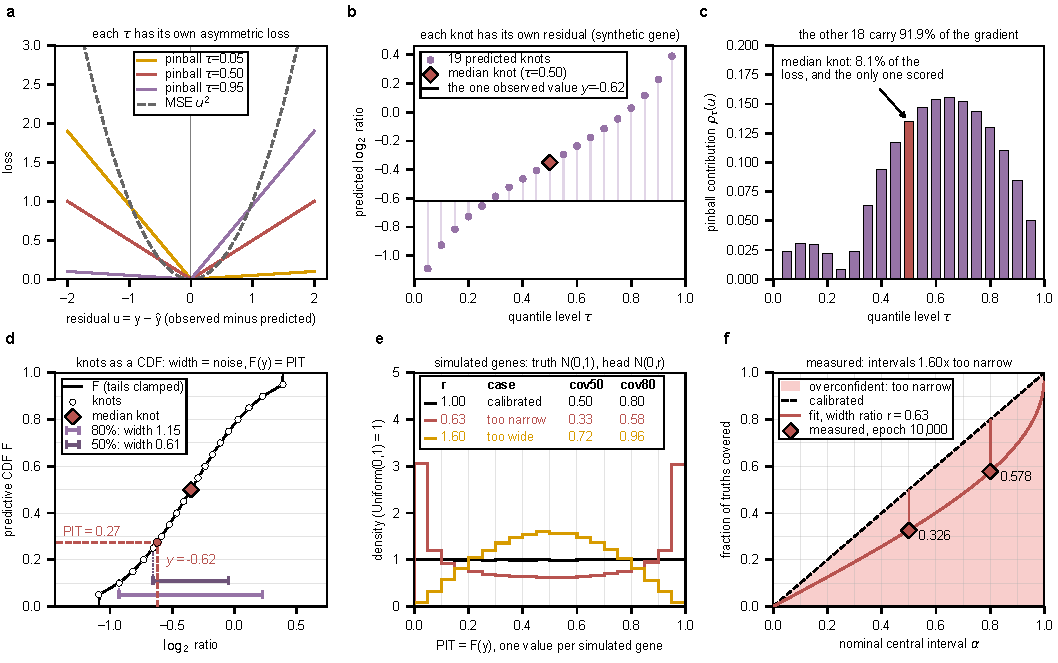
\includegraphics[width=\textwidth]{figures/pinball_vs_mse.pdf}
\caption[]{\textbf{The pinball loss, what its knots carry, and what the metric reads.}
Panels \textbf{a} to \textbf{e} are synthetic; \textbf{f} is measured. \textbf{a},
the pinball loss at three quantile levels against squared error. \textbf{b}, one
illustrative gene: 19 predicted knots, the median knot, and the one observed value; each
knot's residual to that value feeds its own pinball term. \textbf{c}, the 19 terms; the
median carries $8.1\,\%$ and is the only knot the metric scores. \textbf{d}, the same
knots read back as a CDF (joined piecewise-linearly, tails clamped as
\file{_quantile_pit} does): the central 80\,\% and 50\,\% interval widths are the
model's own noise estimate for that gene, and the CDF at the observed value is its PIT.
\textbf{e}, PIT histograms over 200{,}000 simulated genes with truth $N(0,1)$ and a head
predicting $N(0, r)$: flat when $r = 1$, U-shaped when the intervals are too narrow, humped
when too wide, with the coverage of the central 50\,\% and 80\,\% intervals per case.
\textbf{f}, the incumbent's measured coverage at epoch 10{,}000 as a reliability curve;
the fitted curve is a single width ratio $r = 0.63$, derived not measured. Generated by
\file{plot_pinball_vs_mse.py}.}
\label{fig:findings-pinball}
\end{figure}

\subsection{Spread across the long-budget arms is a function of budget, and not a
monotone one\secstatus{todo}}
\label{sec:findings-spread}

The same eight long-budget arms, rescored on the prefix of their own curves
(\file{short_budget_spread.py}). Read every spread below as an arm spread plus
nondeterminism, an upper bound on the replicate spread at that budget:

\begin{table}[htbp]
\centering\small
%% SOURCE: results/short_budget_spread.json, by_budget; the power columns follow from sd at
%% alpha 0.05 and power 0.8 (z_sum 2.8016) for a two-sample contrast.
\begin{tabular}{rrrrrr}
\toprule
epochs & mean & sd & main effect, 32 v 32 & cell, 16 v 16 & arm, 8 v 8 \\
\midrule
   350 & $0.1198$ & $0.0096$ & $0.0067$ & $0.0095$ & $0.0135$ \\
   500 & $0.1223$ & $0.0058$ & & & \\
   700 & $0.1411$ & $0.0166$ & & & \\
 1{,}000 & $0.1609$ & $0.0099$ & & & \\
 1{,}500 & $0.1670$ & $0.0117$ & & & \\
 2{,}000 & $0.1745$ & $0.0151$ & & & \\
 2{,}800 & $0.1821$ & $0.0175$ & & & \\
 4{,}000 & $0.1883$ & $0.0171$ & & & \\
 6{,}000 & $0.1917$ & $0.0177$ & & & \\
 9{,}900 & $0.1965$ & $0.0222$ & & & \\
\bottomrule
\end{tabular}
\caption[]{Mean and spread of the eight long-budget v9 arms at truncated budgets, from
500-sample curves. The spread is not monotone in budget: 700 epochs is the noisiest point
below 2{,}000. The last three columns are the detectable gap at the 350-epoch spread for
the three contrast sizes a $2^4$ grid affords, the same arithmetic that sized the v10 grid
at 1{,}400 epochs and two seeds rather than 700 and four.}
\label{tab:findings-power}
\end{table}

Two traps were hit measuring this and are recorded so the next reader does not hit them:
a resumed run passes an epoch filter and inherits its parent's config, so it masquerades
as a replicate and is identified only by where its curve starts; and a whole-curve-maximum
collapse test reads a run that collapses late as healthy, so collapse is tested on the last
value.

\subsection{A short screen does not rank like a long run, within one configuration
\secstatus{todo}}
\label{sec:findings-rank}

Spearman between the 700-epoch and 3{,}000-epoch \file{roll_max} of the same run
(\file{budget_rank_preservation.py}): $-0.139$, $p = 0.53$, $n = 23$; top-3 overlap one of
three, top-5 one of five. After resume exclusion the corpus is the eight mask-schedule arms
plus the objective round, so this measures persistence among near-identical
configurations: a run's early rank among them says nothing about its late rank. Whether a
short screen orders
different configurations correctly is answerable only on a multi-config corpus, and the
v10 grid (\cref{sec:readouts-factorial}) is the first one.

\subsection{The validation loss bottoms out early and the metric keeps rising
\secstatus{todo}}
\label{sec:findings-lossmin}

Full per-epoch history of every live v9 run whose loss is not the metric, 27 runs of
1{,}000 epochs or more that neither collapsed nor resumed, read 2026-09-09
(\file{loss_min_vs_pearson_peak.py}, \cref{fig:findings-lossmin}); the four
\file{listmle} runs that joined the objective round after \cref{tab:findings-head} was
read are included, and both \file{listmle_mse} runs collapsed. The median epoch of the
\file{val/loss} minimum is 481 (range 203 to 3{,}097) and no run bottoms out by epoch
100. The median final loss sits $9.0\,\%$ above its minimum. Every run's Pearson peak
(median epoch 2{,}433) comes after its loss minimum, at a loss already $6.8\,\%$ above the
floor, and the median Pearson gained between the two is $+0.057$. The long budget buys
Pearson on a rising validation objective, which is the fact the metric-aligned round was
built to confront. The eight Pearson-objective runs are excluded here by construction,
since their loss and metric coincide on train.

\begin{figure}[htbp]
\centering
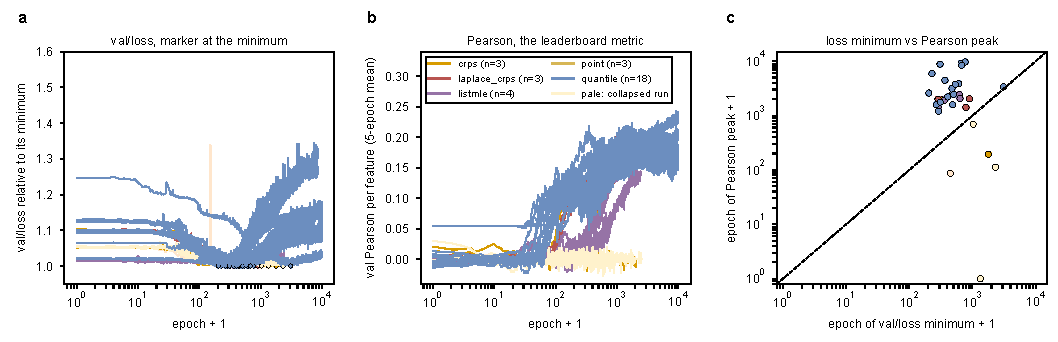
\includegraphics[width=\textwidth]{figures/loss_min_vs_pearson_peak.pdf}
\caption[]{\textbf{Where the loss bottoms out and where the Pearson peaks.} \textbf{a},
validation loss relative to its minimum, one curve per run, colored by head; pale curves
are collapsed runs. \textbf{b},
the 5-epoch rolling mean of validation Pearson. \textbf{c}, the epoch of the loss minimum
against the epoch of the Pearson peak; every point lies above the diagonal. Generated by
\file{loss_min_vs_pearson_peak.py}.}
\label{fig:findings-lossmin}
\end{figure}

\subsection{Every run behind these numbers\secstatus{todo}}
\label{sec:findings-runs}

\Cref{tab:wandb-runs-019} links every run this document draws a number from to its W\&B
page, generated by \file{wandb_run_index.py} from the same result files the sections read.

%% GENERATED by experiments/019-simb-multimodal/scripts/wandb_run_index.py
%% from results/short_budget_spread.json, round_leaderboards.csv,
%% mech_round_readout.csv, pearson_round_readout.csv, v10_grid_factorial.csv.
%% Do not edit by hand; rerun the script.
%% SOURCE: the result files named above (run ids), URLs built from project and id.
\begin{table}[htbp]
  \centering
  \footnotesize
  \caption[W\&B runs behind this document]{Every run behind the numbers in this document, 74 in all, in projects \href{https://wandb.ai/zhao-group/torchcell_019_expr_v9}{\texttt{torchcell\_019\_expr\_v9}} and \href{https://wandb.ai/zhao-group/torchcell_019_expr_v10}{\texttt{torchcell\_019\_expr\_v10}} (entity \texttt{zhao-group}). One row per round and arm; each entry is a seed and its run id, linked to the run page, with the final epoch in brackets. The objective round lists each fresh run and its resume. The v10 grid names cells by embedding, trunk, readout and weight decay.}
  \label{tab:wandb-runs-019}
  \begin{tabular}{@{}llp{0.60\textwidth}@{}}
    \hline
    Round & Arm & Seed: run [epochs] \\
    \hline
    v9 mask arms & \texttt{M\_coarse} & 0: \href{https://wandb.ai/zhao-group/torchcell_019_expr_v9/runs/ebkzn1ao}{\texttt{ebkzn1ao}} [9,900] \\
     & \texttt{M\_fine} & 0: \href{https://wandb.ai/zhao-group/torchcell_019_expr_v9/runs/hx8pxdic}{\texttt{hx8pxdic}} [9,900] \\
     & \texttt{M\_gate\_rezero} & 0: \href{https://wandb.ai/zhao-group/torchcell_019_expr_v9/runs/u1vuznme}{\texttt{u1vuznme}} [9,900] \\
     & \texttt{M\_hi} & 0: \href{https://wandb.ai/zhao-group/torchcell_019_expr_v9/runs/da5g4o9v}{\texttt{da5g4o9v}} [9,900] \\
     & \texttt{M\_lo} & 0: \href{https://wandb.ai/zhao-group/torchcell_019_expr_v9/runs/f2wf23oy}{\texttt{f2wf23oy}} [9,900] \\
     & \texttt{M\_nomix} & 0: \href{https://wandb.ai/zhao-group/torchcell_019_expr_v9/runs/rb3bhryq}{\texttt{rb3bhryq}} [9,900] \\
     & \texttt{M\_off} & 0: \href{https://wandb.ai/zhao-group/torchcell_019_expr_v9/runs/tow1z48n}{\texttt{tow1z48n}} [9,900] \\
     & \texttt{M\_sched} & 0: \href{https://wandb.ai/zhao-group/torchcell_019_expr_v9/runs/8r5ewoaq}{\texttt{8r5ewoaq}} [9,900] \\
    \hline
    objective & \texttt{Q\_point} & 0: \href{https://wandb.ai/zhao-group/torchcell_019_expr_v9/runs/8gklzy7n}{\texttt{8gklzy7n}} [9,895] 0: \href{https://wandb.ai/zhao-group/torchcell_019_expr_v9/runs/iiqohck6}{\texttt{iiqohck6}} [2,039] 1: \href{https://wandb.ai/zhao-group/torchcell_019_expr_v9/runs/yrs7x07y}{\texttt{yrs7x07y}} [9,895] 1: \href{https://wandb.ai/zhao-group/torchcell_019_expr_v9/runs/qplil73c}{\texttt{qplil73c}} [2,039] 2: \href{https://wandb.ai/zhao-group/torchcell_019_expr_v9/runs/y8ex71vn}{\texttt{y8ex71vn}} [9,863] 2: \href{https://wandb.ai/zhao-group/torchcell_019_expr_v9/runs/he2vb4qr}{\texttt{he2vb4qr}} [2,577] \\
     & \texttt{Q\_crps} & 0: \href{https://wandb.ai/zhao-group/torchcell_019_expr_v9/runs/m6utaeu8}{\texttt{m6utaeu8}} [9,526] 0: \href{https://wandb.ai/zhao-group/torchcell_019_expr_v9/runs/lljkhhck}{\texttt{lljkhhck}} [1,995] 1: \href{https://wandb.ai/zhao-group/torchcell_019_expr_v9/runs/djgkdzol}{\texttt{djgkdzol}} [9,895] 1: \href{https://wandb.ai/zhao-group/torchcell_019_expr_v9/runs/nx5dwhp8}{\texttt{nx5dwhp8}} [2,039] 2: \href{https://wandb.ai/zhao-group/torchcell_019_expr_v9/runs/eiu664kx}{\texttt{eiu664kx}} [9,777] 2: \href{https://wandb.ai/zhao-group/torchcell_019_expr_v9/runs/hzumvs8y}{\texttt{hzumvs8y}} [2,031] \\
     & \texttt{Q\_laplace} & 0: \href{https://wandb.ai/zhao-group/torchcell_019_expr_v9/runs/1xa3x8uc}{\texttt{1xa3x8uc}} [9,526] 0: \href{https://wandb.ai/zhao-group/torchcell_019_expr_v9/runs/c981k5n1}{\texttt{c981k5n1}} [1,995] 1: \href{https://wandb.ai/zhao-group/torchcell_019_expr_v9/runs/7v9l6ett}{\texttt{7v9l6ett}} [9,895] 1: \href{https://wandb.ai/zhao-group/torchcell_019_expr_v9/runs/ia6312dv}{\texttt{ia6312dv}} [2,039] 2: \href{https://wandb.ai/zhao-group/torchcell_019_expr_v9/runs/g69wskm0}{\texttt{g69wskm0}} [9,777] 2: \href{https://wandb.ai/zhao-group/torchcell_019_expr_v9/runs/lz8gq5ui}{\texttt{lz8gq5ui}} [2,031] \\
    \hline
    mechanism & \texttt{R\_ref} & 0: \href{https://wandb.ai/zhao-group/torchcell_019_expr_v9/runs/i63dbvha}{\texttt{i63dbvha}} [4,139] 1: \href{https://wandb.ai/zhao-group/torchcell_019_expr_v9/runs/r2s57bvt}{\texttt{r2s57bvt}} [8,499] \\
     & \texttt{R\_basis64} & 0: \href{https://wandb.ai/zhao-group/torchcell_019_expr_v9/runs/h9l8aguy}{\texttt{h9l8aguy}} [8,499] 1: \href{https://wandb.ai/zhao-group/torchcell_019_expr_v9/runs/4gtnrja7}{\texttt{4gtnrja7}} [7,018] \\
     & \texttt{R\_pergene} & 0: \href{https://wandb.ai/zhao-group/torchcell_019_expr_v9/runs/4u0txt3s}{\texttt{4u0txt3s}} [8,499] 1: \href{https://wandb.ai/zhao-group/torchcell_019_expr_v9/runs/vqek7ali}{\texttt{vqek7ali}} [8,499] \\
     & \texttt{R\_pergene\_basis64} & 0: \href{https://wandb.ai/zhao-group/torchcell_019_expr_v9/runs/nrkorko0}{\texttt{nrkorko0}} [4,079] 1: \href{https://wandb.ai/zhao-group/torchcell_019_expr_v9/runs/3qy1rh0o}{\texttt{3qy1rh0o}} [6,589] \\
    \hline
    metric-aligned & \texttt{Q\_pearson} & 0: \href{https://wandb.ai/zhao-group/torchcell_019_expr_v9/runs/zaul43n1}{\texttt{zaul43n1}} [4,091] 1: \href{https://wandb.ai/zhao-group/torchcell_019_expr_v9/runs/kspeoljg}{\texttt{kspeoljg}} [4,074] 2: \href{https://wandb.ai/zhao-group/torchcell_019_expr_v9/runs/p2qq2525}{\texttt{p2qq2525}} [3,166] \\
     & \texttt{Q\_pearson\_mse} & 0: \href{https://wandb.ai/zhao-group/torchcell_019_expr_v9/runs/hsauh7al}{\texttt{hsauh7al}} [4,089] 1: \href{https://wandb.ai/zhao-group/torchcell_019_expr_v9/runs/ppc2pyv5}{\texttt{ppc2pyv5}} [4,077] 2: \href{https://wandb.ai/zhao-group/torchcell_019_expr_v9/runs/4ei42tb1}{\texttt{4ei42tb1}} [3,169] \\
     & \texttt{Q\_pearson\_b64} & 0: \href{https://wandb.ai/zhao-group/torchcell_019_expr_v9/runs/7ylecrjz}{\texttt{7ylecrjz}} [6,345] 1: \href{https://wandb.ai/zhao-group/torchcell_019_expr_v9/runs/wb2xocf2}{\texttt{wb2xocf2}} [6,339] \\
    \hline
    v10 grid & \texttt{c0\_rand\_big\_mlp\_wd0} & 0: \href{https://wandb.ai/zhao-group/torchcell_019_expr_v10/runs/dd26f5nw}{\texttt{dd26f5nw}} [1,399] 1: \href{https://wandb.ai/zhao-group/torchcell_019_expr_v10/runs/nxrpgwca}{\texttt{nxrpgwca}} [1,176] \\
     & \texttt{c1\_ptt5\_big\_mlp\_wd0} & 0: \href{https://wandb.ai/zhao-group/torchcell_019_expr_v10/runs/te8272kk}{\texttt{te8272kk}} [1,399] 1: \href{https://wandb.ai/zhao-group/torchcell_019_expr_v10/runs/l4uw0g1e}{\texttt{l4uw0g1e}} [1,399] \\
     & \texttt{c2\_rand\_small\_mlp\_wd0} & 0: \href{https://wandb.ai/zhao-group/torchcell_019_expr_v10/runs/j5oc0kbf}{\texttt{j5oc0kbf}} [1,399] 1: \href{https://wandb.ai/zhao-group/torchcell_019_expr_v10/runs/zu0mp0ly}{\texttt{zu0mp0ly}} [1,399] \\
     & \texttt{c3\_ptt5\_small\_mlp\_wd0} & 0: \href{https://wandb.ai/zhao-group/torchcell_019_expr_v10/runs/lnoei9xt}{\texttt{lnoei9xt}} [1,399] 1: \href{https://wandb.ai/zhao-group/torchcell_019_expr_v10/runs/wv0qlp4n}{\texttt{wv0qlp4n}} [1,192] \\
     & \texttt{c4\_rand\_big\_lin\_wd0} & 0: \href{https://wandb.ai/zhao-group/torchcell_019_expr_v10/runs/0htrkihg}{\texttt{0htrkihg}} [1,119] 1: \href{https://wandb.ai/zhao-group/torchcell_019_expr_v10/runs/59a4xytq}{\texttt{59a4xytq}} [1,399] \\
     & \texttt{c5\_ptt5\_big\_lin\_wd0} & 0: \href{https://wandb.ai/zhao-group/torchcell_019_expr_v10/runs/6ee07w1j}{\texttt{6ee07w1j}} [1,399] 1: \href{https://wandb.ai/zhao-group/torchcell_019_expr_v10/runs/7ue6aduu}{\texttt{7ue6aduu}} [990] \\
     & \texttt{c6\_rand\_small\_lin\_wd0} & 0: \href{https://wandb.ai/zhao-group/torchcell_019_expr_v10/runs/6ktjsou6}{\texttt{6ktjsou6}} [1,399] 1: \href{https://wandb.ai/zhao-group/torchcell_019_expr_v10/runs/ujbunglx}{\texttt{ujbunglx}} [1,020] \\
     & \texttt{c7\_ptt5\_small\_lin\_wd0} & 0: \href{https://wandb.ai/zhao-group/torchcell_019_expr_v10/runs/dcx8l9z6}{\texttt{dcx8l9z6}} [1,148] 1: \href{https://wandb.ai/zhao-group/torchcell_019_expr_v10/runs/ts735yhp}{\texttt{ts735yhp}} [1,399] \\
     & \texttt{c8\_rand\_big\_mlp\_wd2} & 0: \href{https://wandb.ai/zhao-group/torchcell_019_expr_v10/runs/fk6luj3g}{\texttt{fk6luj3g}} [1,119] 1: \href{https://wandb.ai/zhao-group/torchcell_019_expr_v10/runs/7n0ohmht}{\texttt{7n0ohmht}} [1,399] \\
     & \texttt{c9\_ptt5\_big\_mlp\_wd2} & 0: \href{https://wandb.ai/zhao-group/torchcell_019_expr_v10/runs/5ivl9nat}{\texttt{5ivl9nat}} [1,399] 1: \href{https://wandb.ai/zhao-group/torchcell_019_expr_v10/runs/iyvyd7c3}{\texttt{iyvyd7c3}} [990] \\
     & \texttt{c10\_rand\_small\_mlp\_wd2} & 0: \href{https://wandb.ai/zhao-group/torchcell_019_expr_v10/runs/p2dj91nf}{\texttt{p2dj91nf}} [1,399] 1: \href{https://wandb.ai/zhao-group/torchcell_019_expr_v10/runs/yecoyfgc}{\texttt{yecoyfgc}} [1,029] \\
     & \texttt{c11\_ptt5\_small\_mlp\_wd2} & 0: \href{https://wandb.ai/zhao-group/torchcell_019_expr_v10/runs/oe77kyf6}{\texttt{oe77kyf6}} [1,148] 1: \href{https://wandb.ai/zhao-group/torchcell_019_expr_v10/runs/hhvof18w}{\texttt{hhvof18w}} [1,399] \\
     & \texttt{c12\_rand\_big\_lin\_wd2} & 0: \href{https://wandb.ai/zhao-group/torchcell_019_expr_v10/runs/kt9tezrk}{\texttt{kt9tezrk}} [1,399] 1: \href{https://wandb.ai/zhao-group/torchcell_019_expr_v10/runs/rd64e6kx}{\texttt{rd64e6kx}} [1,170] \\
     & \texttt{c13\_ptt5\_big\_lin\_wd2} & 0: \href{https://wandb.ai/zhao-group/torchcell_019_expr_v10/runs/r9w7i1fw}{\texttt{r9w7i1fw}} [1,399] 1: \href{https://wandb.ai/zhao-group/torchcell_019_expr_v10/runs/c3xrtsr7}{\texttt{c3xrtsr7}} [1,399] \\
     & \texttt{c14\_rand\_small\_lin\_wd2} & 0: \href{https://wandb.ai/zhao-group/torchcell_019_expr_v10/runs/jrwpcoxd}{\texttt{jrwpcoxd}} [1,399] 1: \href{https://wandb.ai/zhao-group/torchcell_019_expr_v10/runs/4ity6oib}{\texttt{4ity6oib}} [1,399] \\
     & \texttt{c15\_ptt5\_small\_lin\_wd2} & 0: \href{https://wandb.ai/zhao-group/torchcell_019_expr_v10/runs/a6mmvj8i}{\texttt{a6mmvj8i}} [1,399] 1: \href{https://wandb.ai/zhao-group/torchcell_019_expr_v10/runs/04204r3z}{\texttt{04204r3z}} [1,198] \\
    \hline
  \end{tabular}
\end{table}


\subsection{Training on the metric does not resolve it\secstatus{todo}}
\label{sec:findings-pearson}

Two heads were added to \file{torchcell/losses/distributional.py} on 2026-09-06:
\file{pearson}, whose loss is one minus the mean per-feature Pearson over the genes hidden
at the current unmasking step, each gene's correlation taken over the strains in the batch
where it is hidden, with columns of fewer than three scored rows or constant prediction or
target dropped as the metric drops them; and \file{pearson_mse}, the same plus the masked
squared error at unit weight as a scale anchor. Both are point-shaped, carry no PIT and
no calibration keys, and the pure loss is scale-free, so its \file{mse}, \file{nmse} and
spread ratio are not comparable to any other arm's. Eighty-six unit tests and a container
canary (\texttt{2375312}) preceded the launch. The readout is \cref{sec:readouts-pearson}:
collapse at every batch-32 seed of the pure loss, at two of three seeds of the anchored
one, and parity with the incumbent for the batch-64 survivors, which peak by epoch 2{,}400
and give part of it back.

A third pair followed on 2026-09-08: \file{listmle}, the Plackett-Luce negative
log-likelihood of the true ordering of the strains in the batch, per hidden gene, divided
by the list length (Xia et al.\ 2008), and \file{listmle_mse}, the same plus the masked
squared error at unit weight. The question it asks is the ranking one: given a set of
knockouts, which strain expresses gene $g$ highest. ListMLE keeps a gradient on a constant
column ($\log(n!)/n$ per gene, where Pearson drops the column), is shift-invariant but not
scale-invariant, so predicted spread can only grow under it, and makes the batch part of
the objective as Pearson does. Ninety-eight unit tests and a canary (\texttt{2385788})
preceded the launch; the readout so far is \cref{sec:readouts-listmle}.

%% notes-tex/019-simb-multimodal-expression/sections/2-readouts.tex
%% SOURCE: experiments/019-simb-multimodal/results/v10_grid_factorial.json (script
%% v10_grid_factorial.py), results/mech_round_readout.json (mech_round_readout.py),
%% results/pearson_round_readout.json (pearson_round_readout.py), and sacct/sstat output
%% for IGB jobs 2369697, 2371531, 2378262, 2378267, 2378268 as recorded in
%% notes/experiments.019-simb-multimodal.expression-strand-retrospective.md. Every score
%% is the leaderboard's roll_max (pull_round_leaderboards.py) on the full per-epoch history.

\section{The readouts, 2026-09-08: three rounds, one large effect\secstatus{todo}}
\label{sec:readouts}

Three rounds returned within two days of each other: the $2^4$ factorial on Delta, the
mechanism round on IGB (both designed in the SIMB retrospective's launch section,
\file{notes-tex/019-simb-multimodal/sections/10-launch.tex}), and the first two days of
the metric-aligned objective round, which trains on $1 - r$ directly
(\cref{sec:findings-pearson}). Every
score below is \file{roll_max}, the maximum of a centered 5-epoch rolling mean of
\file{val/expression/pearson_per_feature}, read from the full per-epoch history, and every
contrast is at a MATCHED budget computed as the smallest final epoch across the runs being
compared. The scoring rule is an upward-biased order statistic; it is the same rule on every
side of every contrast, so the bias cancels in a difference and not in an absolute number.

\subsection{The factorial: embedding content is the only factor that moves the score
\secstatus{todo}}
\label{sec:readouts-factorial}

Job \texttt{21830323} ran 16 cells at two seeds, one run per GPU, four per node. Five of
the eight array tasks completed 1{,}400 epochs; three hit the two-day wall between epochs
990 and 1{,}198, so the matched budget is epochs $\le 990$.

\begin{table}[htbp]
\centering\small
%% SOURCE: results/v10_grid_factorial.json, matched_all (32 runs) and matched_healthy (31)
\begin{tabular}{llrrrr}
\toprule
factor & contrast (level 1 $-$ level 0) & effect & $t$ & effect, 31 runs & $t$ \\
\midrule
embedding    & \file{prot_T5_all} $-$ \file{random_1024} & $+0.068$ & $+7.8$ & $+0.076$ & $+17.3$ \\
trunk        & $L{=}2,h{=}45$ $-$ $L{=}6,h{=}90$     & $-0.012$ & $-1.4$ & $-0.018$ & $-4.0$ \\
readout      & linear $-$ two-layer                   & $+0.007$ & $+0.8$ & $+0.002$ & $+0.5$ \\
weight decay & $10^{-4}$ $-$ $10^{-8}$                & $+0.005$ & $+0.5$ & $-0.000$ & $-0.1$ \\
\midrule
embedding $\times$ trunk & & $+0.017$ & $+2.0$ & $+0.013$ & $+2.9$ \\
\bottomrule
\end{tabular}
\caption[]{Main effects of the v10 grid at epochs $\le 990$, 16 runs a side. The error is the
pooled within-cell replicate standard deviation, $0.0246$ on 16 degrees of freedom over all
32 runs (standard error per effect $0.0087$), and $0.0122$ on 15 degrees of freedom once the
one run that never left the chance band is dropped (standard error $0.0044$). The other five
two-way interactions have $|t| < 1.3$ in both readings.}
\label{tab:readouts-factorial}
\end{table}

\begin{figure}[htbp]
\centering
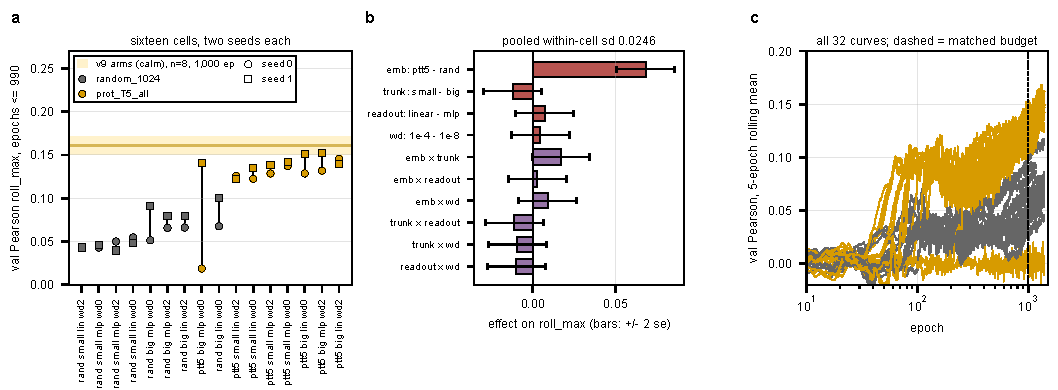
\includegraphics[width=\textwidth]{figures/v10_grid_factorial.pdf}
\caption[]{\textbf{The v10 grid at a matched budget.} \textbf{a}, every cell's two seeds at
epochs $\le 990$, sorted by cell mean and colored by embedding, against the eight
long-budget v9 arms at 1{,}000 epochs ($0.161 \pm 0.010$, \file{calm} embeddings, band is
one standard deviation across arms). \textbf{b}, main effects and two-way
interactions with $\pm 2$ standard errors from the pooled within-cell spread.
\textbf{c}, all 32 validation curves; the dashed line is the matched budget. Generated by
\file{v10_grid_factorial.py}.}
\label{fig:readouts-factorial}
\end{figure}

\pfstep{Embedding content is worth $0.07$, three times the replicate spread.} The ProtT5
cells average $0.129$ against $0.061$ for random vectors of the same width, and no cell of
one level overlaps any cell of the other (\cref{fig:readouts-factorial}a). The contrast was
built as a content test at matched width 1{,}024, so it says the content matters and says
nothing about \file{calm}, the incumbent's embedding, which is not a level of the grid. The
one healthy draw of the incumbent-with-ProtT5 cell scores $0.141$ against the incumbent's
$0.161 \pm 0.010$ at the same budget, one draw against eight, and that is not a resolved gap
in either direction.

\pfstep{Readout width and weight decay are measured nulls.} Both effects are under $0.008$
against a resolution of about $0.02$ at two standard errors. The trunk is a small effect in
favor of the deeper one, $-0.012$ over all runs and $-0.018$ once the stuck run is dropped,
and it is sharper under ProtT5 (the interaction). Of the four factors chosen to act on the
train-validation gap, one acts.

\pfstep{One run in 32 never learned.} Cell 1 seed 0 (\texttt{te8272kk}: ProtT5, $L{=}6$,
two-layer readout, weight decay $10^{-8}$) sits at $0.019$ at its best and $-0.007$ at
epoch 1{,}399 with \file{nmse} $1.010$, while its seed-1 twin is the grid's best single run
at $0.169$. That pair alone carries most of the pooled variance, which is why both readings
are given. Its cause is not measured.

\subsection{The mechanism round: per-gene readout $+0.03$, under the round's resolution
\secstatus{todo}}
\label{sec:readouts-mech}

All four array tasks of the round ended in the cgroup out-of-memory handler at host RSS
61~GB against a 60~GB request, after 3.5 to 4.6 days. In each task one of the two packed
runs was killed and the other finished its 8{,}500 epochs, so the matched budget is set by
the shortest survivor, epochs $\le 4{,}079$. The two seed-1 runs abandoned on cabbi at epoch
${\approx}1{,}595$ when that half moved to the A40 node are superseded, not replicates, and
are dropped.

\begin{table}[htbp]
\centering\small
%% SOURCE: results/mech_round_readout.json, roll_max_le_4079 and paired_contrasts["4079"]
\begin{tabular}{lrrrr}
\toprule
arm & seed 0 & seed 1 & paired difference vs \texttt{R\_ref} (s0 / s1) & mean \\
\midrule
\texttt{R\_ref}               & $0.188$ & $0.169$ & & \\
\texttt{R\_basis64}           & $0.175$ & $0.200$ & $-0.014$ / $+0.030$ & $+0.008$ \\
\texttt{R\_pergene}           & $0.189$ & $0.224$ & $+0.001$ / $+0.054$ & $+0.028$ \\
\texttt{R\_pergene\_basis64}  & $0.214$ & $0.199$ & $+0.026$ / $+0.029$ & $+0.027$ \\
\bottomrule
\end{tabular}
\caption[]{The mechanism round at epochs $\le 4{,}079$, paired within seed against the
in-round reference. Seed 0 ran on cabbi Ada cards, seed 1 on one A40 node, so GPU type is
a seed-level block. The eight long-budget v9 arms score $0.188 \pm 0.017$ at 4{,}000
epochs and both \texttt{R\_ref} draws fall inside that band.}
\label{tab:readouts-mech}
\end{table}

\begin{figure}[htbp]
\centering
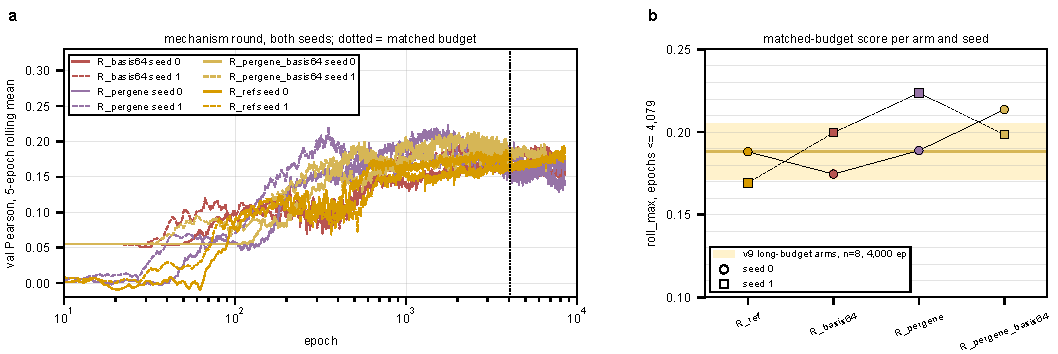
\includegraphics[width=\textwidth]{figures/mech_round_readout.pdf}
\caption[]{\textbf{The mechanism round.} \textbf{a}, validation Pearson of all eight runs
(solid seed 0, dashed seed 1); the dotted line is the matched budget. \textbf{b}, the
matched-budget score per arm and seed against the long-budget arm band at 4{,}000 epochs.
Generated by \file{mech_round_readout.py}.}
\label{fig:readouts-mech}
\end{figure}

\pfstep{The pair term alone is a null.} Its two paired differences disagree in sign and
average $+0.008$. The per-gene readout arms average $+0.027$, and the combined arm is
positive at both seeds, but the round was sized to resolve about $0.06$ at two pairs
(\cref{tab:findings-power}), so this is a direction and not a result. What every curve does
show is the dynamics: the per-gene arms reach their peak between epochs 1{,}200 and 2{,}600
and give part of it back (\texttt{R\_pergene} ends at $0.137$ and $0.170$ against peaks of
$0.189$ and $0.224$), while the reference and basis arms are flat or still rising at 8{,}500.
Whether the give-back is overfitting of the extra per-gene parameters is a hypothesis and
is not measured.

\pfstep{A tagging defect, found in the readout.} The arm script carried a wave-4b
\texttt{R\_ref} branch ahead of the wave-5 one; a shell \texttt{case} takes its first
match, so every reference run of this round is tagged \file{stage-wave4b}. The readout
selects by arm and config tag, and the shadowing branch is removed.

\subsection{The metric-aligned round at day two: collapse is the rule at batch 32
\secstatus{todo}}
\label{sec:readouts-pearson}

Three arms train on $1 - r$ directly, the mean per-feature Pearson over the genes hidden at
the current unmasking step (\file{pearson}), the same plus a masked squared error at unit
weight (\file{pearson_mse}), and the pure loss at batch 64 (\file{pearson_b64}), on IGB cabbi
from 2026-09-06. The two batch-32 arms run three seeds at two runs per card, the batch-64
arm two seeds solo. They were read at 1.9 of their 5 days, so every number here is partial
and the readout script records the epoch reached.

\begin{table}[htbp]
\centering\small
%% SOURCE: results/pearson_round_readout.json, read 2026-09-08 16:40 CT
\begin{tabular}{llrrrrr}
\toprule
arm & seed & epoch & \file{roll_max} @ epoch & last & on the floor from & spread ratio at end \\
\midrule
\file{pearson}     & 0 & 3{,}902 & $0.145$ @ 215   & $0.000$ & 584   & $0.000$ \\
\file{pearson}     & 1 & 3{,}886 & $0.133$ @ 151   & $0.000$ & 2{,}203 & $0.000$ \\
\file{pearson}     & 2 & 3{,}021 & $0.137$ @ 242   & $0.000$ & 680   & $0.000$ \\
\file{pearson_mse} & 0 & 3{,}899 & $0.137$ @ 138   & $0.000$ & 360   & -- \\
\file{pearson_mse} & 1 & 3{,}888 & $0.194$ @ 3{,}193 & $0.168$ & alive & $0.43$ \\
\file{pearson_mse} & 2 & 3{,}023 & $0.035$ @ 5     & $0.000$ & 14    & -- \\
\file{pearson_b64} & 0 & 6{,}051 & $0.194$ @ 1{,}926 & $0.163$ & alive & $0.80$ \\
\file{pearson_b64} & 1 & 6{,}049 & $0.186$ @ 2{,}419 & $0.138$ & alive & $0.73$ \\
\bottomrule
\end{tabular}
\caption[]{The metric-aligned round, partial. ``On the floor from'' is the first epoch after
which the 5-epoch rolling mean of the validation Pearson stays under $0.02$; the seed-1
\file{pearson} run is near zero from epoch ${\approx}250$ and flickers above the line until
2{,}203. The spread ratio is predicted over true standard deviation
(\file{pred_sd_ratio}). The eight long-budget v9 arms score $0.188 \pm 0.017$ at 4{,}000
epochs and $0.192 \pm 0.018$ at 6{,}000.}
\label{tab:readouts-pearson}
\end{table}

\begin{figure}[htbp]
\centering
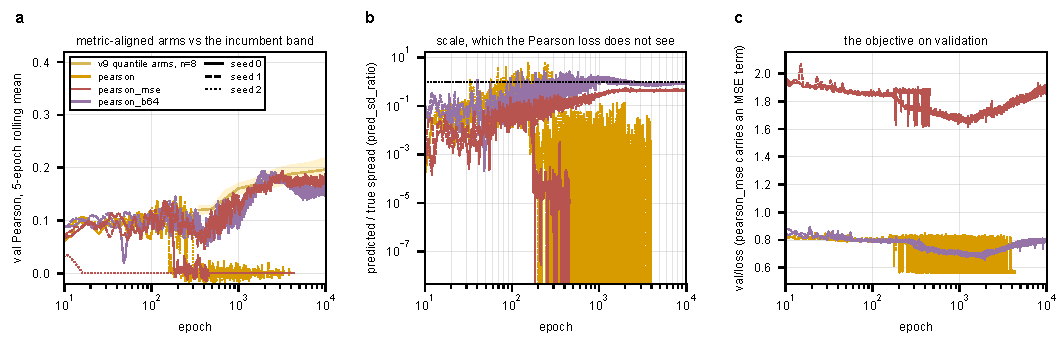
\includegraphics[width=\textwidth]{figures/pearson_round_readout.pdf}
\caption[]{\textbf{The metric-aligned round at day two.} \textbf{a}, validation Pearson of
all eight runs against the incumbent replicate band. \textbf{b}, predicted over true spread,
which the Pearson loss cannot see; a run whose outputs go constant falls off the bottom.
\textbf{c}, the objective on validation; \file{pearson_mse} carries the squared-error term
and sits on its own scale. Generated by \file{pearson_round_readout.py}.}
\label{fig:readouts-pearson}
\end{figure}

\pfstep{Five of six batch-32 runs are on the floor, and the loss does not see it.} The
three pure-Pearson runs peak between $0.13$ and $0.145$ at epochs 150 to 240 and then fall,
their predicted spread dropping from about $0.3$ to $10^{-7}$ over the same epochs
(\cref{fig:readouts-pearson}b): the network's output goes constant per gene. Their
validation loss holds near $0.56$ throughout, because the loss drops a constant column as
invalid and averages over the columns still varying, so it reads $1 - 0.44$ on a handful of
genes while the metric reads $0$ on all of them. The failure mode the design named is the
one that occurred, with the difference that the loss never reads its connected zero. The
squared-error anchor at unit weight did not prevent it: \file{pearson_mse} collapsed by
epoch 14 at one seed and 360 at another, and its surviving seed is alive at $0.194$ and
rising, inside the long-budget arm band.

\pfstep{The batch-64 runs survive and sit on the band, not above it.} Both are at 6{,}050
epochs with spread ratios of $0.73$ and $0.80$, \file{roll_max} $0.194$ and $0.186$
against the incumbent's $0.192 \pm 0.018$ at that budget, peaked near epochs 1{,}900 to
2{,}400 and drifting down since. Batch size and solo placement are confounded in that arm,
so why it survives is not measured; the in-batch correlation being taken over twice as many
strains is a hypothesis. Nothing in the round beats the quantile head at any budget read so
far, and the question it was launched to answer, whether the metric's late rise is
generalization gap or objective disagreement, is answerable only on the live runs after the
wall.

\subsection{Packed five-day runs die of host memory\secstatus{todo}}
\label{sec:readouts-oom}

Four of four packed tasks that ran past three and a half days ended \file{OUT_OF_MEMORY}
(\texttt{2369697} 0--1, \texttt{2371531} 2--3), at \file{MaxRSS} 61.4 and 61.1~GB. The
Pearson-round packed tasks read 21.3~GB at 1.9 days and the solo batch-64 tasks 17.2~GB.
Hypothesis (untested): resident memory grows roughly linearly through a run, in which case
the packed Pearson tasks reach the 60~GB line near day five, at the edge of their wall. What
grows is not identified; the \file{file_system} sharing strategy introduced in
\texttt{f1bfa95b} to stop the file-descriptor exhaustion is the obvious suspect and is
unverified. The memory of a running job cannot be raised, and the two rounds that finished
lost one run per task to it rather than the whole task.

%% notes-tex/019-simb-multimodal-expression/sections/3-next.tex
%% SOURCE: the open-decision entries of
%% notes/experiments.019-simb-multimodal.expression-strand-retrospective.md (2026-09-06 and
%% 2026-09-08); the power figures from results/short_budget_spread.json.

\section{What the evidence leaves open\secstatus{todo}}
\label{sec:next}

Each item is a decision the measurements above do not make, stated with the measurement
that would.

\pfstep{Which number is the target.} Stopping on the validation loss says every run is done
by epoch 300 to 700 and the long-budget campaign is over; stopping on Pearson says the
curves have not turned at 19,000 (\cref{sec:findings-lossmin}). The manuscript reports
Pearson and the objective is the pinball loss, and the metric-aligned round shows the
naive resolution, training on Pearson, is unstable at batch 32 and no better than the
incumbent at batch 64 (\cref{sec:readouts-pearson}). The decision is about what the paper
claims, not about what to run.

\pfstep{The incumbent's embedding against ProtT5.} The grid measured content against
random at width 1{,}024 and did not include \file{calm}
(\cref{sec:readouts-factorial}). A two-arm replicate set at the incumbent configuration,
\file{calm} against \file{prot_T5_all}, three seeds each at 1{,}000 epochs where the
replicate spread is $0.0099$, resolves a gap of about $0.02$ and is the cheapest contrast
left on the table: six runs of under a day each.

\pfstep{The per-gene readout at a resolving replicate count.} $+0.027$ at two pairs against a
resolution of $0.06$ (\cref{sec:readouts-mech}). Detecting $0.03$ at the 4{,}000-epoch
spread of $0.0171$ needs about six pairs; at 1{,}000 epochs and $0.0099$ it needs three.
Whether the arm's early peak and give-back survive a shorter budget is what a 1{,}000-epoch
replicate would also show.

\pfstep{The Pearson round.} The three cabbi cards holding collapsed batch-32 runs can be
freed now or left to the wall on 2026-09-11; the packed tasks cannot be partially
canceled without killing their live sibling, and the live \file{pearson_mse} seed sits in
one of them. The batch-64 runs are the only informative survivors and are solo.

\pfstep{Packing.} Four of four packed five-day tasks died of host memory
(\cref{sec:readouts-oom}). Until the growth is identified, a five-day arm is either solo on
its card or budgeted at 48~GB per run rather than 30, and either choice halves the slots
the launch arithmetic assumed.

\pfstep{The per-gene mean on squared error.} No live run beats \file{nmse} $= 1$ at its
Pearson peak (\cref{sec:findings-state}). The retrospective's one-parameter rescale
argument has not been applied to any run of the campaign; it costs nothing and would say
whether the campaign's models are, like the sprint's, spread $1.8\times$ wider than their
correlation justifies.


\end{document}
